\documentclass[12pt,a4paper]{article}

% 1. Encoding and Core Language
\usepackage[T1]{fontenc}
\usepackage[utf8]{inputenc}
\usepackage[english]{babel}
\usepackage{csquotes}
\usepackage{xcolor} % Loaded early to avoid conflicts with TikZ

% 2. Math and Physics (Load before table packages)
\usepackage{amsmath}
\allowdisplaybreaks
\usepackage{amssymb}
\usepackage{amsfonts}

% 3. Graphics and TikZ
\usepackage{graphicx}
\usepackage{caption}
\usepackage{tikz}
\usetikzlibrary{positioning, arrows.meta, shapes.geometric, shadows, patterns}

% 4. Bibliography (Must come before hyperref)
\usepackage[
    backend=biber, 
    style=ieee,
    maxnames=3,
    giveninits=true,
    sorting=none,
    doi=true,
    isbn=false,
    sortcites,
]{biblatex}

% 5. Tables (Specific order: array -> booktabs -> tabularx -> longtable -> xltabular)
\usepackage{array}
\usepackage{booktabs}
\usepackage{multirow}
\usepackage{colortbl}
\usepackage{tabularx}
\usepackage{longtable}
\usepackage{xltabular}
\usepackage{pdflscape}
\usepackage{float}

% 6. Layout
\usepackage{geometry}
\geometry{left=2cm,right=2cm,top=2cm,bottom=2cm}
\setlength{\parindent}{0pt}

% 7. THE FINALE: Referencing (Order is mandatory!)
% \usepackage{url}
% \usepackage[
%     unicode=true, 
%     hidelinks, 
%     colorlinks=true, 
%     allcolors=blue,
%     bookmarks=true,         % Enables bookmarks
%     bookmarksnumbered=true, % Shows the section numbers in the navigation
%     bookmarksopen=true      % Opens the sidebar by default when the PDF is opened
% ]{hyperref}
% \usepackage[capitalize, noabbrev]{cleveref}
\usepackage[unicode=true]{hyperref} % enables use of metadata for pdfs and hyperlinks within a document
\hypersetup{%colorlinks=true
% activate this part for the boxes 
colorlinks=false, %flag for prints
pdfborder={0 0 1}, % thickness of box
linkbordercolor={1 0 0},
% activate this part to not have the boxes
% hidelinks,  % this option would hide links for the print version of your thesis
% linkcolor=red!35!black,    %definition of the link color
% citecolor=green!35!black,  %definition of the cite color
% urlcolor=magenta!35!black, %definition of the url color
pdfauthor=Simon Kraft, % Optional: Specify the author of the pdf
pdftitle=Assignment 1   % Optional: Specify the title within the pdf
} 
\usepackage[capitalize,noabbrev]{cleveref}
% \usepackage{bookmark}

\addbibresource{references.bib}

\usepackage[utf8]{inputenc}
\usepackage{array} % For better table row heights


% \addbibresource{references.bib} % Note the .bib extension is required here

% --- Document Metadata ---
\title{
    \vspace{5em}
    \large \textbf{CPSC 644 - Computer Networks} \\

    \huge \textbf{Assignment 1} \\
}

\author{
    \large Submitted by \\[0.2cm]
    \renewcommand{\arraystretch}{1.5}
    \begin{tabular}{|c|c|}
        \hline
        \textbf{Student ID} & \textbf{Name} \\
        \hline
        230171256 & Simon Kraft \\
        \hline
    \end{tabular}
}

\date{\today}

\begin{document}

\maketitle
\newpage

\section*{Exercise 1}

Consider a packet of length $L$ that begins at end system A and travels over three links to the destination end system. These three links are connected by \textit{two} packets switches. Let $d_i, s_i, \text{ and } R_i$ denote the length, propagation speed, and the transmission rate of link $i \in \{1, 2, 3\}$. The packet switches delay each packet by $d_{\text{proc}}$.

\medskip

\textit{Hint: the processing delay is the same for each switch and there are no queuing delays.}

\subsection*{a)}

\textbf{Question:} What is the total end-to-end delay in terms of $d_i, s_i, R_i \text{ and } d_{\text{proc}}$?

\bigskip

The network considered in this exercise is drawn in~\cref{fig:ex1-network-topology}.

\vspace{1em}

\begin{figure}[H]
    \centering
        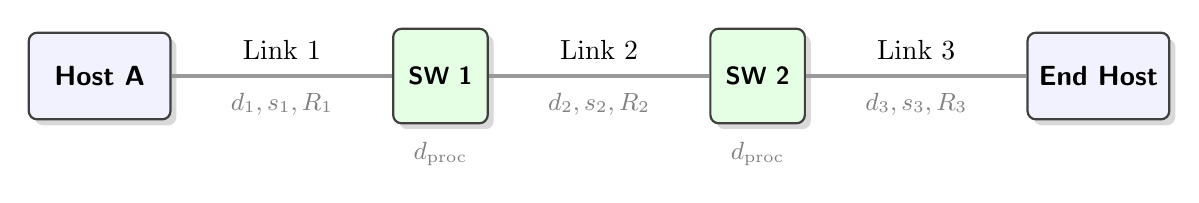
\begin{tikzpicture}[
        node distance=2.8cm,
        % Modern Host Style
        host/.style={
            rectangle, draw=darkgray, thick, 
            fill=blue!5, rounded corners=3pt,
            minimum width=1.8cm, minimum height=1.1cm,
            drop shadow={opacity=0.3}, % Adds depth
            font=\sffamily\bfseries
        },
        % Modern Switch Style (Visualized with the "X" cross pattern)
        router/.style={
            rectangle, draw=darkgray, thick,
            fill=green!10, rounded corners=3pt,
            minimum size=1.2cm,
            drop shadow={opacity=0.3},
            font=\sffamily\small\bfseries
        },
        % Link style: Simple thick line, no arrow at the front
        link/.style={
            draw=gray!80, line width=1.5pt
        },
        % Optional: indicator for d_proc
        proc/.style={text=red!70!black, font=\footnotesize\itshape}
    ]

        % Nodes
        \node[host] (A) {Host A};
        \node[router, right=of A] (S1) {SW 1};
        \node[router, right=of S1] (S2) {SW 2};
        \node[host, right=of S2] (B) {End Host};

        % Switch Symbols (Standard networking icons often have a cross)
        % \draw[gray, thin] (S1.45) -- (S1.225) (S1.135) -- (S1.315);
        % \draw[gray, thin] (S2.45) -- (S2.225) (S2.135) -- (S2.315);

        % Connections (No arrows)
        \draw[link] (A) -- node[above=2pt, black] {Link 1} 
                         node[below=2pt, gray] {\small $d_1, s_1, R_1$} (S1);
        \draw[link] (S1) -- node[above=2pt, black] {Link 2} 
                          node[below=2pt, gray] {\small $d_2, s_2, R_2$} (S2);
        \draw[link] (S2) -- node[above=2pt, black] {Link 3} 
                          node[below=2pt, gray] {\small $d_3, s_3, R_3$} (B);

        % Annotations for d_proc
        \node[below=0.1cm of S1, gray] {\small $d_{\text{proc}}$};
        \node[below=0.1cm of S2, gray] {\small $d_{\text{proc}}$};

    \end{tikzpicture}
    \vspace{-1em}
    \caption{Drawing of Network Topology}
    \label{fig:ex1-network-topology}
\end{figure}

\vspace{1em}

To calculate the end-to-end delay, we need to calculate the delay for each single hop on the way from Host A to the End Host. This nodal delay can be expressed by the formula:

\[
    d_{\text{nodal}} = d_{\text{proc}} + d_{\text{queue}} + d_{\text{trans}} + d_{\text{prop}}
\]

where:

\begin{itemize}
    \item $d_{\text{proc}}$: nodal processing delay (e.g. check for bit errors, check headers)
    \item $d_{\text{queue}}$: queueing delay (waiting at output link for transmission)
    \item $d_{\text{trans}}$: transmission delay (time to transmit packet onto link)
    \item $d_{\text{prop}}$: propagation delay (time for packet to completely propagate from one hop to next)
\end{itemize}

Furthermore, transmission and propagation delay can be calculated using the above given link lengths $d_i$, propagation speeds $s_i$, and transmission rates $R_i$ for all links $i \in \{1, 2, 3 \}$ and the packet lenght $L$.

\[
    d_{\text{trans}}^{(i)} = \frac{L}{R_i} \qquad \qquad d_{\text{prop}}^{(i)} = \frac{d_i}{s_i}
\]

\vspace{0.5em}

As processing delay $d_{\text{proc}}$ is the same for each packet switch and there are no queueing delays, the formula to calculate the end-to-end delay in this scenario is given by:

\begin{equation}
    \begin{aligned}
        d_{\text{end-to-end}} &= 2 \cdot d_{\text{proc}} \;+\; \sum_{i=1}^3 \frac{L}{R_i} \;+\; \sum_{i=1}^3 \frac{d_i}{s_i} \\[0.25em]
        d_{\text{end-to-end}} &= 2 \cdot d_{\text{proc}} \;+\; \sum_{i=1}^3 d_{\text{trans}}^{(i)} \;+\; \sum_{i=1}^3 d_{\text{prop}}^{(i)}
    \end{aligned}
    \label{eq:end-to-end-delay}
\end{equation}

\vspace{0.5em}

The transmission delay needs to be included for each link, as the links do not directly push incoming bits through. Instead, the routers work in a store-and-forward way, meaning the entire packet needs to arrive at router before it can be transmitted on the next link.

\subsection*{b)}

\textbf{Question:} For the given values, what is the end-to-end delay?

\bigskip

\[
    \begin{aligned}
        L &= 1,500 \text{ bytes } = 12,000 \text{ bits} \\[0.5em]
        \forall i \in \{1, 2, 3\}: s_i &= 2.5 \cdot 10^8 \text{ m/s} = 2.5 \cdot 10^5 \text{ km/s} \\[0.5em]
        \forall i \in \{1, 2, 3\}: R_i &= 2.5 \text{ Mbps} = 2,500,000 \text{ bps} \\[0.5em]
        d_{\text{proc}} &= 3 \text{ ms} = 0.003 \text{ s} \\[0.5em]
        d_1 = 5,000 \text{ km} \quad d_2 &= 4,000 \text{ km} \quad d_3 = 1,000 \text{ km}
    \end{aligned}
\]

\vspace{1.5em}


To calculate the end-to-end delay we use Equation~\ref{eq:end-to-end-delay} from the previous exercise:

\[
    \begin{aligned}
        d_{\text{end-to-end}} &= 2 \cdot 0.003 \text{ s} + 3 \cdot \frac{12,000 \text{ bits}}{2,500,000 \text{ bits/s}} + \frac{5,000 \text{ km} + 4,000 \text{ km} + 1,000 \text{ km} }{2.5 \cdot 10^5 \text{ km/s}} \\[0.75em]
        &= 0.006 \text{ s} + 0.0144 \text{ s} + 0.04 \text{ s} = \mathbf{0.0604} \text{ s} 
    \end{aligned}
\]

\vspace{1em}

The end-to-end delay in this scenario is $0.0604$ seconds.

\subsection*{c)}

\textbf{Question:} What is the end-to-end delay formula, when there is no processing delay, the transmission rate is the same for all hops ($R$), and the packet switch doesn't store-and-forward?

\bigskip

As a receiver of data can immediately start transmitting the bits it received again onto the next link, there is only the transmission delay from the Host A to push all the bits of the packet onto the first link. Therefore, the other transmission delays are not existent in this scenario. \\

Furthermore, as there is no processing delay, i.e. $d_{\text{proc}}=0$, the final formula changes to:

\begin{equation}
    \begin{aligned}
        d_{\text{end-to-end}} &= 2 \cdot d_{\text{proc}} \;+\; \frac{L}{R} \;+\; \sum_{i=1}^3 \frac{d_i}{s_i} \\[0.25em]
        d_{\text{end-to-end}} &= \frac{L}{R} \;+\; \sum_{i=1}^3 \frac{d_i}{s_i}
    \end{aligned}
\end{equation}

\section*{Exercise 2}

In modern packet-switched networks, including the Internet, the source host segments long, application-layer messages (for example, an image or a music file) into smaller packets and sends the packets into the network. The receiver then reassembles the packets back into the  original message. We refer to this process as message segmentation. \\

Figure~\ref{fig:message-segmentation} shows the end-to-end transport with and without message segmentation. In this example, the message $L$ sent from source to destination is $10^6$ bits long and each link has 5 Mbps. Propagation, queueing, and processing delay are ignored.

\vspace{1.5em}

\begin{figure}[H]
    \centering
    \includegraphics[width=0.6\textwidth]{exercise2_img.png}
    \caption{End-to-end message transport. a) without message segmentation and b) with message segmentation.}
    \label{fig:message-segmentation}
\end{figure}

\subsection*{a)}

\textbf{1. Question:}  How long does it take to move the message from the source host to the first packet switch without message segmentation?

\bigskip

Information that we have:

\begin{itemize}
    \item Transmission happens at $R = 5 \text{ Mbps} = 5,000,000 \text{ bits/s}$.
    \item Store-and-forward is used, i.e. entire packet must arrive at switch before forwarding
    \item Formula for calculating transmission delay $\frac{L}{R}$
    \item $L = 10^6 \text{ bits} = 1,000,000 \text{ bits}$
\end{itemize}

\vspace{1em}

Therefore, moving from source to the first packet switch takes:

\[
    d_{\text{1-hop}} = \frac{L}{R} = \frac{1,000,000 \text{ bits}}{5,000,000 \text{ bits/s}} = \mathbf{0.2} \text{ s}
\]

\vspace{0.5em}

\textbf{2. Question:} What is the total time to move the message from source host to destination host?

\bigskip

As we have have 3 links, the whole packet needs to be transmitted 3 times. Therefore the total is given by:

\[
    d_{\text{total}} = 3 \cdot \frac{L}{R} = 3 \cdot \frac{1,000,000 \text{ bits}}{5,000,000 \text{ bits/s}} = \mathbf{0.6} \text{ s}
\]

\subsection*{b)}

\textbf{Setup:} Message segmented in 100 packets, each size 10,000 bits. \\

\textbf{1. Question:} How long does it take to move the first packet from source host to the first switch? 

\bigskip

As the transmission rate remains equal and the number of bits reduced to 10,000, the result is:

\[
    d_{\text{first-packet-at-1-hop}} = \frac{L}{R} = \frac{10,000 \text{ bits}}{5,000,000 \text{ bits/s}} = \mathbf{0.002} \text{ s}
\]

\vspace{0.5em}

\textbf{2. Question:} At what time will the second packet be fully received at the first switch?

\bigskip

As the transmission of the second packet begins, when the first packet is fully transmitted (after 0.002 seconds), we just need to add the transmission time for the second packet (also 10,000 bits large) onto that:

\[
    d_{\text{second-packet-at-1-hop}} = 0.002 + \frac{L}{R} = 0.002 + \frac{10,000 \text{ bits}}{5,000,000 \text{ bits/s}} = \mathbf{0.004} \text{ s}
\]

\subsection*{c)}

\textbf{Question:} How long does it take to move the file from source host to the destination host when message segmentation is used?

\bigskip

To answer this, we need to determine, when the last packet gets transmitted by the source host and sum it up with the time, it takes for the last packet to go through all 3 links to the destination host:

\[
    \begin{aligned}
        d_{\text{last-packet-at-destination}} &= \underbrace{99 \cdot \frac{10,000 \text{ bits}}{5,000,000 \text{ bits/s}}}_{%
            \substack{\text{Point of time, when} \\
                \text{transmission of last packet starts}
            }} \;+\; \underbrace{3 \cdot \frac{10,000 \text{ bits}}{5,000,000 \text{ bits/s}}}_{%
            \substack{\text{3 transmission delays until} \\
            \text{last packet arrives at destination}
        }} \\[0.5em]
        &= 102 \cdot 0.002 \text{ s} = \mathbf{0.204} \text{ s}
    \end{aligned}
\]

\textbf{Comparison:} of this result with the result from section a).

\bigskip

With message segmentation we are able to reduce the time it takes to transmit the whole data to the destiantion from $0.6$ seconds to $0.204$ seconds. This equals to a reduction of end-to-end delay by almost 66\%. \\

In general, increasing the number of hops also increases the benefits of message segmentation. Without message segmentation, each hops adds another $\frac{L}{R}$ seconds to the total end-to-end delay. With message segmentation, each hops adds only $\frac{l}{R}$ seconds where $l$ is only the size of one single packet. Conversely, decreasing the number of hops, reduces this advantage of message segmentation. With only a single link, sending a message with and without segmentation takes equally long.

\subsection*{d)}

\textbf{Advantages of Message Segmentation}

\begin{itemize}
    \item \textbf{Error Recovery:} when the buffer of a packet switch is full or when there is a bit error in an incoming packet, this packet gets dropped. This can especially happen if large packets arrive at the switch. Dropped packets will then need to be retransmitted. With message segmentation, the system only needs to worry about the specific packet that got dropped, not about the entire message.
    \item \textbf{Sharing Switches:} A single large message blocks the link for a long time. During this time the traffic from other hosts cannot be served. With message segmentation, packets from different sources can be interleaved more easily, so that more people can fairly share the resources of the switch.
\end{itemize}

\subsection*{e)}

\textbf{Disadvantages of Message Segmentation}

\begin{itemize}
    \item \textbf{Encapsulation:} Each packet must have its own header attached to it when it goes down the protocol stack. Sending all these headers increases the total amount of data to be sent, bandwidth is therefore wasted on administrative data rather than on actual payload data.
    \item \textbf{Message Reassembly:} Not all packets of a segmented message take the same path throughout the network. Therefore, the destination host must use compute power and memory to hold this data in a buffer and to later reassemble it correctly before an application can use them.
\end{itemize}

\section*{Exercise 3}

Perform a traceroute between source and destination on the same continent at three different hours of the day.

\begin{figure}[H]
    \centering
    \textbf{5 PM}

    \vspace{0.5em}

    \includegraphics[width=0.85\textwidth]{local_traceroute/5pm.png}
    
    \vspace{1em}

    \textbf{11 PM}
    
    \vspace{0.5em}

    \includegraphics[width=0.85\textwidth]{local_traceroute/11pm.png}

    \vspace{1em}

    \textbf{12 PM}
    
    \vspace{0.5em}

    \includegraphics[width=0.85\textwidth]{local_traceroute/12pm.png}

    \caption{Traceroute of \url{harvard.edu} for three different hours of the day.}
    \label{fig:local-traceroute}
\end{figure}

\subsection*{a)}

The sample average and standard deviation are given by:

\[
    \bar{x} = \frac{1}{n} \sum_{i=1}^{3} x_i \qquad \qquad s = \sqrt{\frac{1}{n-1} \sum_{i=1}^3 (x_i - \bar{x})^2}
\]

With this, we can calculate the following:

\begin{align*}
    \bar{x}_{\text{5-PM}} &= \frac{23.190 + 39.053 + 23.580}{3} = \mathbf{28.608} \\[0.25em]
    s_{\text{5-PM}} &= \sqrt{\frac{(23.190 - 28.608)^2 + (39.053 - 28.608)^2 + (23.580 - 28.608)^2}{2}} = \mathbf{9.048} \\[0.25em]
    \bar{x}_{\text{11-PM}} &= \frac{23.680 + 23.265 + 23.120}{3} = \mathbf{23.355} \\[0.25em]
    s_{\text{11-PM}} &= \sqrt{\frac{(23.680 - 23.355)^2 + (23.265 - 23.355)^2 + (23.120 - 23.355)^2}{2}} = \mathbf{0.291} \\[0.25em]
    \bar{x}_{\text{12-PM}} &= \frac{41.508 + 38.641 + 26.387}{3} = \mathbf{35.512} \\[0.25em]
    s_{\text{12-PM}} &= \sqrt{\frac{(41.508 - 35.512)^2 + (38.641 - 35.512)^2 + (26.387 - 35.512)^2}{2}} = \mathbf{8.031} \\[0.25em]
\end{align*}

\subsection*{b)}

Number of routers in the path for each of the three hours:

\begin{itemize}
    \item \textbf{5 PM}: 13 routers
    \item \textbf{11 PM}: 13 routers
    \item \textbf{12 PM}: 13 routers
\end{itemize}

For each of the three hours, the traceroute command passes through 13 routers until it reaches its destination.

\subsection*{c)}

\textbf{Number of ISPs}

\bigskip

As the routing for the three different hours is always quite similar, we can assume the $\mathbf{4}$ different ISPs:

\begin{itemize}
    \item \textbf{Hop 1-4}: Local institutional network of UNBC
    \item \textbf{Hop 5}: BCNET (network for higher education and research in BC)
    \item \textbf{Hop 6}: \textbf{* * *} the router did not respond to traceroute (often due to security reasons)(no ISP)
    \item \textbf{Hop 7-11}: Shawcable commercial ISP operator
    \item \textbf{Hop 12-13}: Automattic network of destination
\end{itemize}

\vspace{0.5em}

\textbf{Largest Delay}

\bigskip

The largest increases in delay actually seems to appear when going from the BCNET ISP to the Shawcable ISP. Within the Shawcable ISP there are only small increases in the delay, that can be explained through the large distance between British Columbia and Harvard University. Furthermore, the delays in the 12 PM screenshot vary a lot, e.g. one delay at the BCNET ISP takes around 1100 ms, where as the final delay at the destination is still between 26 and 42 ms.

\subsection*{d)}

Perform a traceroute between source and destination on a different continent at three different hourse of the day.

\begin{figure}[H]
    \centering
    \textbf{5 PM}

    \vspace{0.5em}

    \includegraphics[width=0.85\textwidth]{global_traceroute/5pm.png}
    
    \vspace{1em}

    \textbf{11 PM}
    
    \vspace{0.5em}

    \includegraphics[width=0.85\textwidth]{global_traceroute/11pm.png}

    \vspace{1em}

    \textbf{1 PM}
    
    \vspace{0.5em}

    \includegraphics[width=0.85\textwidth]{global_traceroute/1pm.png}

    \caption{Traceroute of \url{uni-bonn.de} for three different hours of the day.}
    \label{fig:global-traceroute}
\end{figure}

\textbf{Averages and standard deviations}

\begin{align*}
    \bar{x}_{\text{5-PM}} &= \frac{148.966 + 148.321 + 148.438}{3} = \mathbf{148.575} \\[0.25em]
    s_{\text{5-PM}} &= \sqrt{\frac{(148.966-148.575)^2 + (148.321-148.575)^2 + (148.438-148.575)^2}{2}} = \mathbf{0.344} \\[0.25em]
    \bar{x}_{\text{11-PM}} &= \frac{183.623 + 154.111 + 151.92}{3} = \mathbf{163.218} \\[0.25em]
    s_{\text{11-PM}} &= \sqrt{\frac{(183.623-163.218)^2 + (154.111-163.218)^2 + (151.92-163.218)^2}{2}} = \mathbf{17.705} \\[0.25em]
    \bar{x}_{\text{1-PM}} &= \frac{149.186 + 148.691 + 148.644}{3} = \mathbf{148.8403} \\[0.25em]
    s_{\text{1-PM}} &= \sqrt{\frac{(149.186-148.8403)^2 + (148.691-148.8403)^2 + (148.644-148.8403)^2}{2}} = \mathbf{0.300}\\[0.25em]
\end{align*}

\textbf{Number of routers}

\begin{itemize}
    \item \textbf{5 PM}: terminated after 33 routers but only until the 17th there were useful responses (further packets probably lost in firewall)
    \item \textbf{11 PM}: terminated after 19 routers but last useful response at 17th router 
    \item \textbf{1 PM}: terminated after 22 routers but last useful at 17th router
\end{itemize}

For each of the three hours, we seemed to have reached our destination (dfn.de) after 17 routers. After that we are just stuck in a firewall and the traceroute packets are not returning to us anymore.

\vspace{1em}

\textbf{Number of ISPs}

\bigskip

As the routing for the three different hours is quite similar, we can assume the $\mathbf{5}$ different ISPs:

\begin{itemize}
    \item \textbf{Hop 1-4}: Local institutional network of UNBC
    \item \textbf{Hop 5}: BCNET
    \item \textbf{Hop 6-12}: Canarie ISP (formerly Canadian Network for the Advancement of Research, Industry and Education)
    \item \textbf{Hop 13-15/16}: GEANT ISP (European Academic Network)
    \item \textbf{Hop 16/17-end}: DFN (German Research Network)
\end{itemize}

\vspace{0.5em}

\textbf{Largest Delay}

\bigskip

The largest increase in delay is observed when going from the Canarie ISP in New York City to the GEANT ISP, by almost doubling the delay due to the trans-oceanic link between North America and Europe which causes a ''long'' propagation time. The delays within Europe don't increase too much.

\section*{Exercise 4}

Use the HTTP/1.1 specification in RFC 2616~\cite{rfc2616} to answer the following questions.

\subsection*{a)}

\textbf{Mechanism between Client and Server to close a persistent connection}

\begin{itemize}
    \item “If either the client or the server sends the close token in the connection header, that request becomes the last one for that connection”~\cite{rfc2616}
    \item Once the closing header is sent, both parties understand that the TCP connection should be closed after the current message got fully transmitted
\end{itemize}


\printbibliography

\end{document}